\section{Teorien: sju proposisjonar}
\label{sec:theory-nn}

Teorien er presentert som sju nummererte proposisjonar med underproposisjonar. Kvar underproposisjon er merka: \textit{d} (definisjon), \textit{a} (postulat), \textit{t} (teorem) eller \textit{o} (observasjon).

\subsection{Proposisjon 1: Formverda er alt som er tilfelle}

Eit \textbf{objekt} er den enklaste bestanddelen i ei form; udeleleg innanfor det valde analysenivået. Ein \textbf{konfigurasjon} er ei samansetjing av objekt; forma er strukturen til konfigurasjonen.

\textbf{Morforommet} til ein klasse er mengda av alle hennar moglege konfigurasjonar \parencite{Raup1966, Mitteroecker2009}. Kvart realisert objekt okkuperer eitt punkt i dette rommet. Det empiriske morforommet er alltid ein projeksjon; forma eksisterer uavhengig av målinga.

Klassen er definert av ein delt \textbf{affordansestruktur} \parencite{Gibson1979}: objekta tilbyr same konstellasjon av operasjonar til same konstellasjon av agentar. Klassen set grensene for morforommet; seleksjonstrykka fordelar innhaldet.

Morforommet ber algebraisk struktur. Formene er lukka under union, differanse og transformasjon. Lat $S$ vere ei mengd av former i eit euklidsk rom $E^n$:

\begin{center}
\begin{tabular}{l@{\hspace{8mm}}l}
$s_1 + s_2$ & union (sum) \\
$s_1 - s_2$ & differanse \\
$s_1 \cdot s_2 := s_1 - (s_1 - s_2)$ & snitt (avleidd) \\
$\tau(a) \leq s, \quad \tau \in \mathrm{Trans}(E^n)$ & innleiring \\
\end{tabular}
\end{center}

\noindent Ei \textbf{innleiring} av $a$ i $s$ er ein transformasjon som plasserer $a$ i $s$ \parencite{Stiny1972, Stiny2006}. Innleiringa er ein eigenskap ved den noverande forma, uavhengig av korleis ho vart konstruert.

Morforommet deler seg i tre regionar: \textbf{busette} (det historiske arkivet), \textbf{opne} (det tilstøytande moglege), og \textbf{forbodne} (utelukka av vilkåra). Desse svarar til ein epistemisk partisjon \parencite{Hatchuel2003, Hatchuel2009}: det \textbf{kjende} ($K$), det \textbf{tenkelege} ($C \setminus K$), og det utenkjelege.

\subsection{Proposisjon 2: Ikkje alle posisjonar er like sannsynlege}

Eit \textbf{seleksjonstrykk} endrar sannsynsfordelinga i morforommet. Trykket er ein gradient, inga regel. Det avgrensar kvar posisjonen \textit{ikkje} kan vere. Forma er det som står att når trykka har utelukka alt anna \parencite{Michl1995}.

Fleire seleksjonstrykk verkar samstundes. Minst to peikar i motstridande retningar; kvar realisert form er difor eit kompromiss. Affordansestrukturen er konstant innanfor klassen og ber null informasjon om kvifor éi form oppstod framfor ei anna. Dei resterande seleksjonstrykka driv all formvariasjon.

\textbf{Materialaffordansen} er operasjonane materialet tillèt og hindrar \parencite{Gibson1979}. Signaturen er latent: han bind sannsynsfordelinga utan å tvinge geometrien.

\subsection{Proposisjon 3: Seleksjonstrykka produserer eit landskap}

\textbf{Tilpassingslandskapet} er vektorsummen av alle verksame seleksjonstrykk \parencite{Wright1932, Waddington1957}. Landskapet har talrike lokale maksima. Stabiliteten til ein haug svarar til brattleiken på dalveggane; dominante trykk tvingar fram \textbf{kanalisering} \parencite{Waddington1957}.

Ein \textbf{stilart} er forma si sverming kring eit felles tyngdepunkt \parencite{Kubler1962}. Stilarten er ein sverm, ikkje ein kategori; grensene er naudsynleg uskarpe.

\subsection{Proposisjon 4: Landskapet er dynamisk}

Seleksjonstrykka kviler aldri. Endringa er diskontinuerleg: lange periodar med stase brotnar i brå skifte \parencite{ElredgeGould1972}. Landskapet har \textbf{minne} \parencite{Arthur1994}; kvar realisert form endrar seleksjonstrykka for den neste. Morforommet ekspanderer kumulativt. Når eitt trykk dominerer, kollapsar landskapet mot éin attraktor. Ei lære som reduserer alle trykk til eitt kollapsar lyskjegla til éin dimensjon. Formene som oppstår under eit kollapsa landskap sviktar under dei reelle trykka læra var blind for.

\subsection{Proposisjon 5: Det finst agentar}

Ein \textbf{agent} er ein operator definert av trippelet: måltilstand, avstandsmåling, justeringsmekanisme \parencite{Rosenblueth1943, Wiener1948, Ashby1956}. Agens krev berre organisering; verken medvit, intensjon eller nervesystem.

Den \textbf{kognitive lyskjegla} er delmengda av morforommet agenten kan representere og manipulere \parencite{Fields2022}. \textbf{Formgrammatikken} \parencite{Stiny1972} utfører diskrete overgangar i formalgebraen. Reglar fyrer på innleiring; inndatageometrien er einaste premiss.

\textbf{Omsorg} er mengda av aksar i morforommet agenten aktivt representerer og justerer for \parencite{Doctor2024}. Kompetansen veks med omsorga. Det me kallar intelligens, er nettopp denne kompetansen. Omsorg er intelligensen sitt innhald; intelligens er omsorga si form.

\subsection{Proposisjon 6: Forma oppstår mellom agentane}

Kvar form er eit \textbf{poly-agentisk kompromiss}. Agens er \textbf{multiskalar} \parencite{Levin2022}. Formproduksjon er distribuert $C \leftrightarrow K$-ekspansjon utført av grammatikkoperasjonar over kompetanseskalaer:

\begin{equation*}
\mathrm{Form} = SG\!\left(\nabla_{C(A)}\, L(c,\, t)\right)
\end{equation*}

\noindent der $SG$ er grammatikken, $\nabla_{C(A)}$ er gradienten avgrensa til lyskjegla, og $L(c,t)$ er landskapet. Forma er grammatikken sin respons på den gradienten agenten kan sjå.

Ein stilart manglar kausal kraft \parencite{Kubler1962, Michl1995}; han er eit \textbf{mønsterminne}, ikkje ei kraft. Inga form er endeleg. Berre den generative strukturen varer: morforom, trykk, landskap, agentar.

\subsection{Proposisjon 7: Forma viser kor langt omsorga rakk}

Talet på aksar agenten aktivt representerer avgjer dimensjonaliteten til kompromisset. Ei form designa under trong omsorg sviktar langs aksar som aldri vart teke vare på. Kvar realisert form er difor eit arkiv over omsorg: kva trykk vart representerte, kva agentar vart koordinerte, kva dimensjonar vart tekne vare på. Forma viser kor langt omsorga rakk.

Figur~\ref{fig:architecture} oppsummerer den fullstendige teoretiske arkitekturen: det empiriske morforommet (A), tilpassingslandskapet avleidd frå det (B), dei nøsta kognitive lyskjeglene over kompetanseskalaer (C), og syntese-likninga som sameinar dei tre kjeldetradisjonane (D).

% Figure 1: The Architecture of Formlaere — composite 4-panel
% A+B from Python (PDF), C+D from TikZ

\begin{figure*}[!t]
\centering

% ── TOP ROW: Data panels ──
\begin{minipage}[t]{0.48\textwidth}
\centering
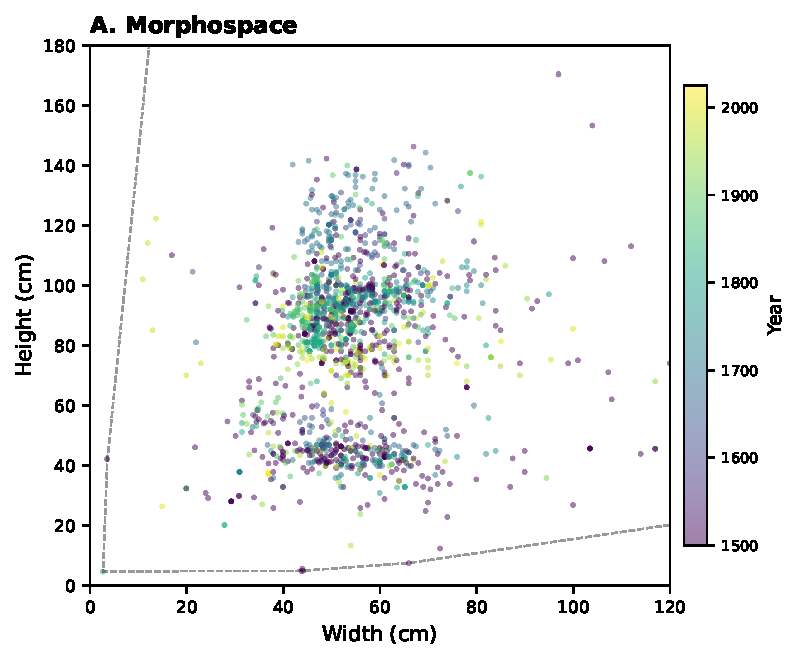
\includegraphics[width=\textwidth]{figures/fig-2-morphospace.pdf}
\end{minipage}%
\hfill
\begin{minipage}[t]{0.48\textwidth}
\centering
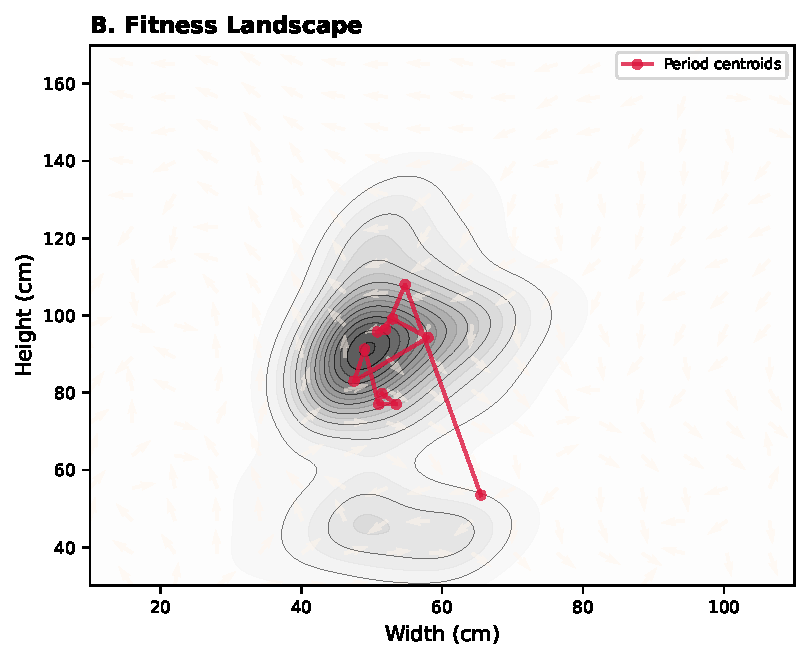
\includegraphics[width=\textwidth]{figures/fig-3-landscape.pdf}
\end{minipage}

\vspace{6pt}

% ── BOTTOM ROW: Structural panels ──
\begin{minipage}[t]{0.48\textwidth}
\centering
{\small\bfseries C.\enspace Multi-Scale Agency}\\[4pt]
\begin{tikzpicture}[
  scale=0.72, transform shape,
  cone/.style={draw=black!60, fill=black!4, thick},
  agent/.style={font=\scriptsize, text=black},
  label/.style={font=\tiny, text=black!70},
  >={Stealth[length=3pt]}
]
\draw[cone, fill=black!3] (-3.0, 0) -- (0, 4.8) -- (3.0, 0) -- cycle;
\node[agent, anchor=west] at (2.1, 0.3) {Market};
\node[label, anchor=west] at (2.1, 0.0) {decade};
\draw[cone, fill=black!5] (-2.2, 0) -- (0, 4.8) -- (2.2, 0) -- cycle;
\node[agent, anchor=west] at (1.5, 0.9) {Designer};
\node[label, anchor=west] at (1.5, 0.6) {month};
\draw[cone, fill=black!7] (-1.5, 0) -- (0, 4.8) -- (1.5, 0) -- cycle;
\node[agent, anchor=west] at (0.9, 1.6) {Tool};
\node[label, anchor=west] at (0.9, 1.3) {hour};
\draw[cone, fill=black!9] (-0.9, 0) -- (0, 4.8) -- (0.9, 0) -- cycle;
\node[agent, anchor=west] at (0.4, 2.4) {Material};
\node[label, anchor=west] at (0.4, 2.1) {minute};
\draw[cone, fill=black!12] (-0.35, 0) -- (0, 4.8) -- (0.35, 0) -- cycle;
\node[agent, anchor=east] at (-0.05, 3.2) {Cell};
\node[label, anchor=east] at (-0.05, 2.9) {ms};
\filldraw[black] (0, 4.8) circle (2pt);
\draw[decorate, decoration={brace, amplitude=4pt, mirror}, black!50]
  (-3.2, -0.1) -- (-3.2, 4.9) node[midway, left=6pt, font=\scriptsize, text=black!70, rotate=90, anchor=south] {cognitive cone $C(A)$};
\draw[<->, black!50] (-3.0, -0.5) -- (3.0, -0.5)
  node[midway, below, font=\scriptsize] {care $= \dim C(A)$};
\end{tikzpicture}
\end{minipage}%
\hfill
\begin{minipage}[t]{0.48\textwidth}
\centering
{\small\bfseries D.\enspace The Synthesis}\\[4pt]
\begin{tikzpicture}[
  scale=0.72, transform shape,
  box/.style={draw=black, rounded corners=3pt, minimum width=26mm, minimum height=8mm,
              font=\small, align=center, thick},
  pillar/.style={draw=#1, fill=#1!8, rounded corners=2pt, minimum width=22mm,
                 minimum height=6mm, font=\scriptsize, align=center},
  >={Stealth[length=3pt]}
]
\node[pillar=teal] (syn) at (-2.4, 4.2) {\textsc{Syntax}\\[-1pt]\tiny Stiny};
\node[pillar=orange!80!black] (log) at (0, 4.2) {\textsc{Logic}\\[-1pt]\tiny Hatchuel \& Weil};
\node[pillar=purple!70!black] (dyn) at (2.4, 4.2) {\textsc{Dynamics}\\[-1pt]\tiny Levin};
\node[box, minimum width=68mm, fill=black!5] (eq) at (0, 2.6)
  {$\mathrm{Form} = SG\!\left(\nabla_{C(A)}\, L(c,\,t)\right)$};
\node[box, fill=teal!8, draw=teal, minimum width=20mm] (sg) at (-2.4, 1.0) {$SG$\\[-2pt]\tiny grammar};
\node[box, fill=orange!8, draw=orange!80!black, minimum width=20mm] (lc) at (0, 1.0) {$L(c,t)$\\[-2pt]\tiny landscape};
\node[box, fill=purple!8, draw=purple!70!black, minimum width=20mm] (ca) at (2.4, 1.0) {$\nabla_{C(A)}$\\[-2pt]\tiny cone};
\node[box, fill=black!8, minimum width=46mm] (form) at (0, -0.4)
  {\textbf{Form} $x \in M(c)$};
\node[font=\small\itshape, text=black!80] (care) at (0, -1.4)
  {care $= \dim C(A)$};
\draw[->, thick, teal] (syn) -- (eq);
\draw[->, thick, orange!80!black] (log) -- (eq);
\draw[->, thick, purple!70!black] (dyn) -- (eq);
\draw[->, thick, teal] (eq) -- (sg);
\draw[->, thick, orange!80!black] (eq) -- (lc);
\draw[->, thick, purple!70!black] (eq) -- (ca);
\draw[->, thick] (sg) -- (form);
\draw[->, thick] (lc) -- (form);
\draw[->, thick] (ca) -- (form);
\draw[->, dashed, thick, black!50] (form.east) -- ++(1.0, 0) |- (lc.east)
  node[pos=0.25, right, font=\tiny, text=black!60] {$K$ expands};
\end{tikzpicture}
\end{minipage}

\caption{The architecture of \formlaere{}. \textbf{A}: 1,662 European chairs projected into morphospace (width $\times$ height); color encodes date. \textbf{B}: Fitness landscape as kernel density estimate with gradient vector field and period centroid trajectory (red). \textbf{C}: Nested cognitive cones across five competence scales; cone width corresponds to care dimensionality. \textbf{D}: The synthesis equation; three source traditions converge on the core equation; dashed arrow shows $K$-expansion feedback.}
\label{fig:architecture}
\end{figure*}


\begin{table*}[!b]
\centering
\caption{Dei sju hovudproposisjonane i \formlaere{} med formelt apparat introdusert av kvar.}
\label{tab:propositions}
\small
\begin{tabularx}{\textwidth}{@{}c >{\raggedright}p{0.28\textwidth} >{\raggedright}p{0.32\textwidth} >{\raggedright\arraybackslash}p{0.22\textwidth}@{}}
\toprule
\textbf{Nr.} & \textbf{Proposisjon} & \textbf{Formelt apparat} & \textbf{Kjeldetradisjon} \\
\midrule
1 & Formverda er alt som er tilfelle & Morforom, algebra, $C$-$K$-partisjon & Stiny; Hatchuel \& Weil \\[3pt]
2 & Ikkje alle posisjonar er like sannsynlege & Seleksjonstrykk, affordanse & Gibson; Michl \\[3pt]
3 & Trykka produserer eit landskap & Tilpassingslandskap, kanalisering & Wright; Waddington \\[3pt]
4 & Landskapet er dynamisk & Stiavhengigheit, tilstøytande mogleg & Arthur; Kauffman \\[3pt]
5 & Det finst agentar & $A := (g,d,\delta)$;\; omsorg $= \dim C(A)$ & Levin; Doctor et al. \\[3pt]
6 & Forma oppstår mellom agentane & $\mathrm{Form} = SG(\nabla_{C(A)} L)$ & Syntese \\[3pt]
7 & Forma viser kor langt omsorga rakk & Diagnostisk konklusjon & --- \\
\bottomrule
\end{tabularx}
\end{table*}
